\subsection{Hydrogen Cryotarget}\label{sec:clas.tgt}


The target used by \g12 was a conical shaped as shown in Fig.~\ref{fig:clas.targetblueprint}. The target was constructed of 0.127$\mu$m thick Kapton and is 40~cm in length and 2~cm in radius, while the incident photon beam had a radius of 1.5~cm. The target cell design shown in Fig,~\ref{fig:clas.targetblueprint} and Fig.~\ref{fig:clas.targetcell} had been used in several experiments and is capable of containing a number of different materials, such as helium, deuterium and hydrogen. For \g12 the target was filled with liquid hydrogen ($\ell$H$_2$). Periodically within each run of \g12, the temperature and pressure of the target was measured and recorded. In Sec~\ref{sec:analysis:systematic}, these measurements will be used to calculate the density of the liquid Hydrogen which is an important quantity to extract cross-section measurements. No polarization on the target was implemented for \g12.

\begin{figure}[h!]\begin{center}
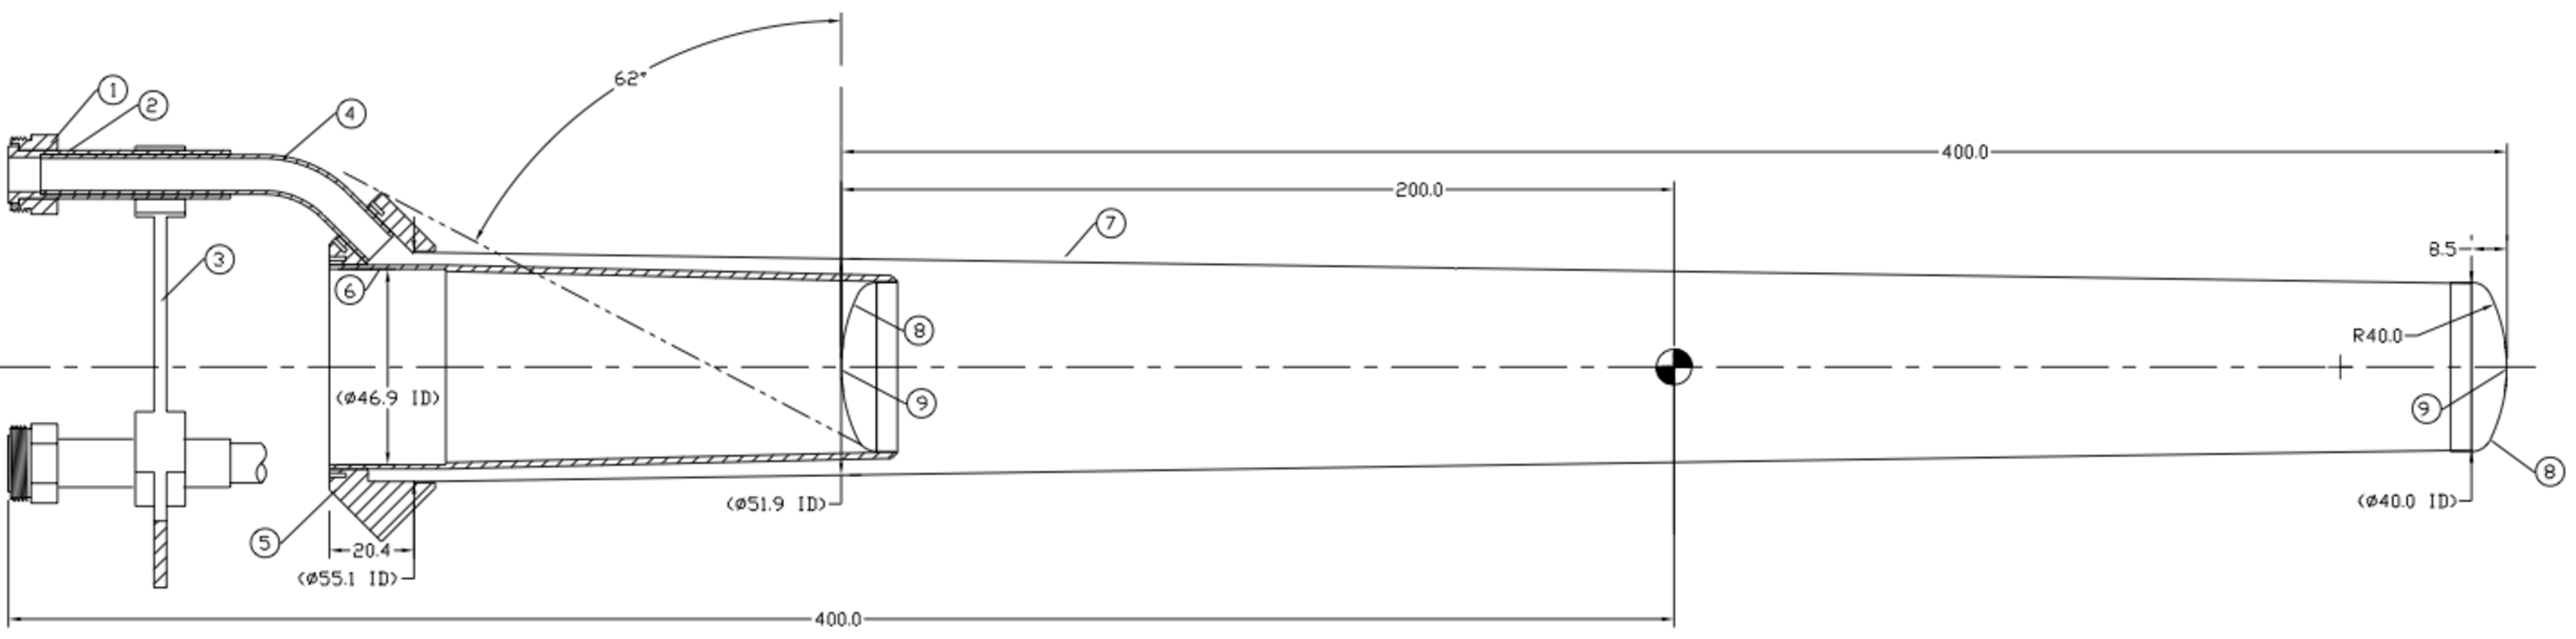
\includegraphics[width=\figwidth,height = \qfigheight]{\grpath/hall-b/g11_target_cell_blueprint.pdf}
\caption[\g12 Target schematic]{\label{fig:clas.targetblueprint}Blueprint schematic of the conical Kapton target cell used for \g12.}
\end{center}\end{figure}

\begin{figure}[h!]\begin{center}
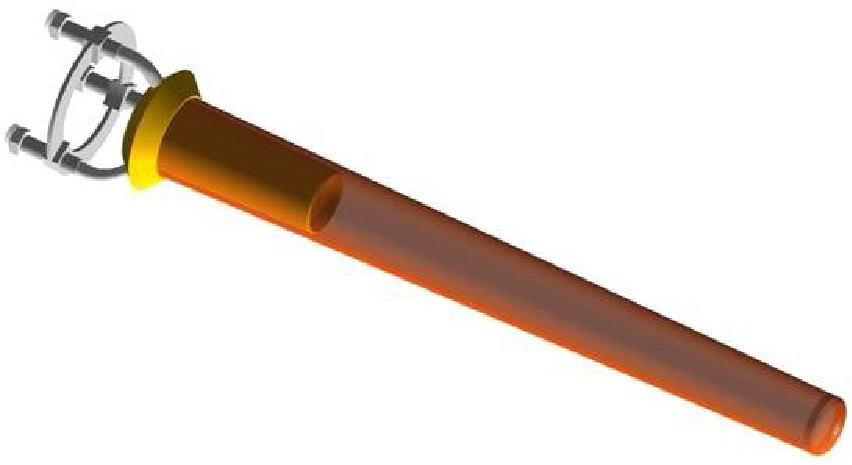
\includegraphics[width=0.6\figwidth]{\grpath/hall-b/g11_target_cell.pdf}
\caption[\g12 Target]{\label{fig:clas.targetcell}The 40~cm long conical Kapton target cell used for \g12.}
\end{center}\end{figure}

%\subsubsection{Target Position for \g12}\label{sec:clas.tgt.position}
The target placement for \g12 was 90~cm upstream of \abbr{CLAS} center, see Fig.~\ref{fig:clas.ced}.
Placing the target at this position increased the forward acceptance from 8$^\circ$  to 6$^\circ$ from the beam-line in the lab frame. However, this placement also decreased large angle acceptance from approximately 140$^\circ$ to 100$^\circ$ in the lab frame. This reduction in large angle acceptance sacrificed large momentum-transfer events where the final state particles were more than about 70$^\circ$ away.
%as well as a reduction in \abbr{DC} resolution. The \abbr{DC} resolution decrease was due to the oblique angle the tracks made with the detector planes.
